\documentclass[12pt, oneside]{article}
\usepackage[letterpaper, margin=1in, headsep=0.5in, left=0.3in, right=2.5in]{geometry}
\usepackage[english]{babel}
\usepackage[utf8]{inputenc}
\usepackage{amsmath}
\usepackage{amsfonts}
\usepackage{amssymb}
\usepackage{tikz}
\usepackage{yhmath}
\usetikzlibrary{quotes, angles}
\usepackage{graphicx}
\usepackage{enumitem}
\usepackage{multicol}

\newif\ifmeta
\metatrue %print standards and topics tags

\title{Regents Geometry}
\author{Chris Huson}
\date{April 2022}

\usepackage{fancyhdr}
\pagestyle{fancy}
\fancyhf{}
\renewcommand{\headrulewidth}{0pt} % disable the underline of the header
\raggedbottom

%\fancyhead[LE]{\thepage}
\fancyhead[RO]{Name:}
\fancyhead[LO]{BECA / Dr. Huson / Geometry Regents Mixed Review}
\cfoot{\thepage}

\begin{document}
\subsubsection*{11.2 Regents: Similar triangles \hfill HSG.SRT.B.5}
\begin{enumerate}[itemsep=1.7cm]
%\subsubsection*{Similarity \hfill January 2020}
\item Triangle $JGR$ is similar to triangle $MST$. Which statement is \emph{not}
always true?
\begin{multicols}{2}
  \begin{enumerate}
    \item $\angle J \cong \angle M$
    \item $\angle G \cong \angle T$ 
    \item $\angle R \cong \angle T$
    \item $\angle G \cong \angle S$
  \end{enumerate}
\end{multicols}

\item In trapezoid $ABCD$ below, $\overline{AB} \parallel \overline{CD}$.
\begin{center}
  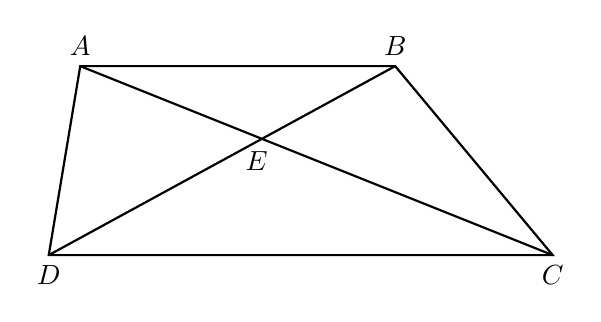
\begin{tikzpicture}[scale=0.8]
    \draw [-, thick] 
      (0,0)node[below]{$D$}--
      (8,0)node[below]{$C$}--
      (5.5,3)node[above]{$B$}--
      (0.5,3)node[above]{$A$}--cycle;
    \draw [-, thick] (0,0)--(5.5,3);
    \draw [-, thick] (0.5,3)--(8,0);
    \node at (3.3, 1.5){$E$};
  \end{tikzpicture}
  \end{center}
If $AE=5.2$, $AC=11.7$, and $CD=10.5$, what is the length of $\overline{AB}$, to \emph{the nearest tenth}?

\item The line represented by $2y=x+8$ is dilated by a scale factor
of $k$ centered at the origin, such that the image of the line has an
equation of $y - \frac{1}{2} x=2$. What is the scale factor?

\item In quadrilateral $ABCD$ below, $\overline{AB} \parallel \overline{CD}$, and $E$, $H$, and $F$ are the midpoints of $\overline{AD}$, $\overline{AC}$,  and $\overline{BC}$, respectively.
\begin{center}
  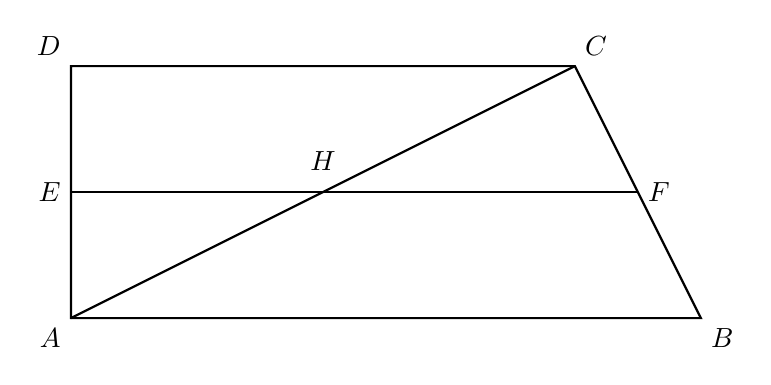
\begin{tikzpicture}[scale=0.8]
    \draw [-, thick] 
      (0,0)node[below left]{$A$}--
      (10,0)node[below right]{$B$}--
      (8,4)node[above right]{$C$}--
      (0,4)node[above left]{$D$}--cycle;
    \draw [-, thick] (0,0)--(8,4);
    \draw [-, thick] (0,2)node[left]{$E$}--(9,2)node[right]{$F$};
    \node at (4,2.5){$H$};
  \end{tikzpicture}
  \end{center}
If $AB=24$, $CD=18$, and $AH=10$, then what is $FH$?

\newpage
\item Given right triangle $ABC$ with a right angle at $C$, $m\angle B=61^\circ$. Given right triangle $RST$ with a right angle at $T$, $m\angle R=29^\circ$.
  \begin{center}
    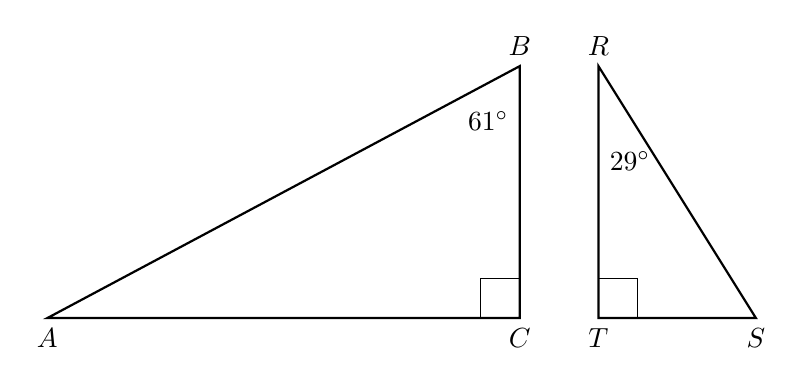
\begin{tikzpicture}[scale=1]
    \draw [thick]
      (0,0)node[below]{$T$}--
      (2,0)node[below]{$S$}--
      (0,3.2)node[above]{$R$}--cycle;
      \draw (0,0)++(0.5,0)--++(0,0.5)--+(-0.5,0);
    \draw [thick]
      (-7,0)node[below]{$A$}--
      (-1,3.2)node[above]{$B$}--
      (-1,0)node[below]{$C$}--cycle;
      \draw (-1,0)++(-0.5,0)--++(0,0.5)--+(0.5,0);
      \node at (-1.4,2.5){$61^\circ$};
      \node at (0.4,2.0){$29^\circ$};
  \end{tikzpicture}
  \end{center}
Which proportion in relation to $\triangle ABC$ and $\triangle RST$ is \emph{not} correct?
  \begin{multicols}{2}
    \begin{enumerate}
      \item $\displaystyle \frac{AB}{RS} = \frac{RT}{AC}$
      \item $\displaystyle \frac{BC}{ST} = \frac{AB}{RS}$ 
      \item $\displaystyle \frac{BC}{ST} = \frac{AC}{RT}$
      \item $\displaystyle \frac{AB}{AC} = \frac{RS}{RT}$
    \end{enumerate}
  \end{multicols}

\item In the accompanying diagram of right triangle $ABC$, altitude $\overline{BD}$ is drawn to hypotenuse $\overline{AC}$.
  \begin{center}
    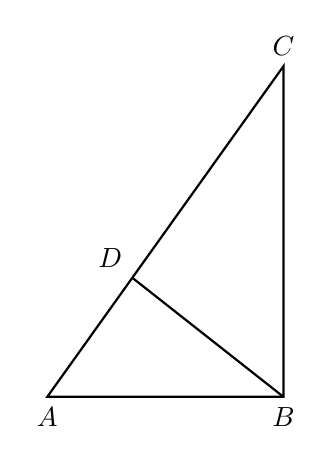
\begin{tikzpicture}[scale=0.6]
    \draw [thick]
    (0,0)node[below]{$A$}--
    (5,0)node[below]{$B$}--
    (5,7)node[above]{$C$}--cycle;
    \draw [thick](1.8,2.52)node[above left]{$D$}--(5,0);
  \end{tikzpicture}
  \end{center}
  Which statement must be true?
  \begin{multicols}{2}
    \begin{enumerate}
      \item $\displaystyle \frac{AD}{AB} = \frac{BC}{AC}$
      \item $\displaystyle \frac{AD}{AB} = \frac{AB}{AC}$ 
      \item $\displaystyle \frac{BD}{BC} = \frac{AB}{AD}$
      \item $\displaystyle \frac{AB}{BC} = \frac{BD}{AC}$
    \end{enumerate}
  \end{multicols}

\newpage
\item In right triangle $RST$ below, altitude $\overline{SV}$ is drawn to hypotenuse $\overline{RT}$.
  \begin{center}
    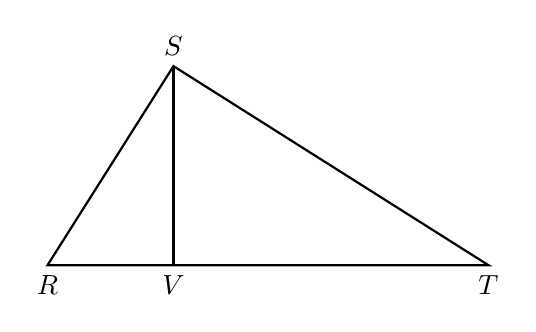
\begin{tikzpicture}[scale=0.8]
    \draw [thick]
    (0,0)node[below]{$R$}--
    (7,0)node[below]{$T$}--
    (2,3.16)node[above]{$S$}--cycle;
    \draw [thick](2,0)node[below]{$V$}--(2,3.16);
  \end{tikzpicture}
  \end{center}
If $RV=4.1$ and $TV=10.2$, what is the length of $\overline{ST}$, to the \emph{nearest tenth}?

\item In the diagram below of right triangle $ABC$, altitude $\overline{BD}$ is drawn to hypotenuse $\overline{AC}$.
  \begin{center}
    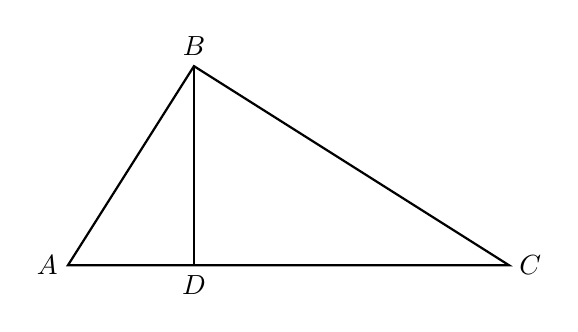
\begin{tikzpicture}[scale=0.8]
    \draw [thick]
    (0,0)node[left]{$A$}--
    (7,0)node[right]{$C$}--
    (2,3.16)node[above]{$B$}--cycle;
    \draw [thick](2,0)node[below]{$D$}--(2,3.16);
  \end{tikzpicture}
  \end{center}
If $BD=4$, $AD=x-6$, and $CD=x$, what is the length of $\overline{CD}$?

\item In the diagram below of $\triangle HAR$ and $\triangle NTY$, angles $H$ and $N$ are right angles, and $\triangle HAR \sim \triangle NTY$
  \begin{center}
    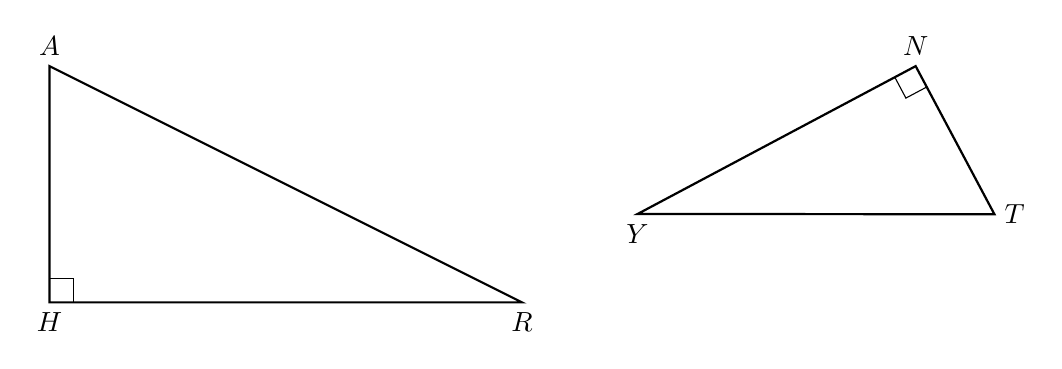
\begin{tikzpicture}[scale=1]
    \draw [thick, xshift=4cm, yshift=2cm, rotate=208]
      (0,0)node[above]{$N$}--
      (4,0)node[below]{$Y$}--
      (0,2.13)node[right]{$T$}--cycle;
      \draw [xshift=4cm, yshift=2cm, rotate=208]
        (0,0)++(0.3,0)--++(0,0.3)--+(-0.3,0);
    \draw [thick]
      (-1,-1)node[below]{$R$}--
      (-7,2)node[above]{$A$}--
      (-7,-1)node[below]{$H$}--cycle;
      \draw (-7,-1)++(0.3,0)--++(0,0.3)--+(-0.3,0);
  \end{tikzpicture}
  \end{center}
If $AR=13$ and $HR=12$, what is the measure of $\angle Y$, to the \emph{nearest degree}?

\newpage
\item In the diagram below of right triangle $KMI$, altitude $\overline{IG}$ is drawn to hypotenuse $\overline{KM}$.
  \begin{center}
    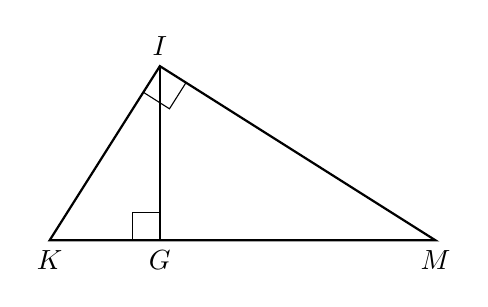
\begin{tikzpicture}[scale=0.7]
    \draw [thick]
    (0,0)node[below]{$K$}--
    (7,0)node[below]{$M$}--
    (2,3.16)node[above]{$I$}--cycle;
    \draw (2,3.16)++(-0.15*2,-0.15*3.16)--++(0.15*3.16,-0.15*2)--+(0.15*2,0.15*3.16);
    \draw [thick](2,0)node[below]{$G$}--(2,3.16);
    \draw (2,0)++(-0.5,0)--++(0,0.5)--+(0.5,0);
  \end{tikzpicture}
  \end{center}
IF $KG=9$ and $IG=12$, what is the length of $\overline{IM}$?


\item In diagram below of right triangle $ABC$, altitude $\overline{BD}$ is drawn.
  \begin{center}
    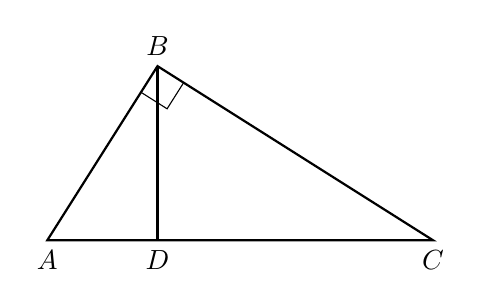
\begin{tikzpicture}[scale=0.7]
    \draw [thick]
    (0,0)node[below]{$A$}--
    (7,0)node[below]{$C$}--
    (2,3.16)node[above]{$B$}--cycle;
    \draw (2,3.16)++(-0.15*2,-0.15*3.16)--++(0.15*3.16,-0.15*2)--+(0.15*2,0.15*3.16);
    \draw [thick](2,0)node[below]{$D$}--(2,3.16);
  \end{tikzpicture}
  \end{center}
Which ratio is always equivalent to $\cos A$?
\begin{multicols}{2}
  \begin{enumerate}
    \item $\displaystyle \frac{AB}{BC}$
    \item $\displaystyle \frac{BD}{BC}$ 
    \item $\displaystyle \frac{BD}{AB}$
    \item $\displaystyle \frac{BC}{AC}$
  \end{enumerate}
\end{multicols}

\item In the diagram of $\triangle ABC$ below, points $D$ and $E$ are on sides $\overline{AB}$ and $\overline{CB}$ respectively, such that $\overline{DE} \parallel \overline{AC}$.
\begin{center}
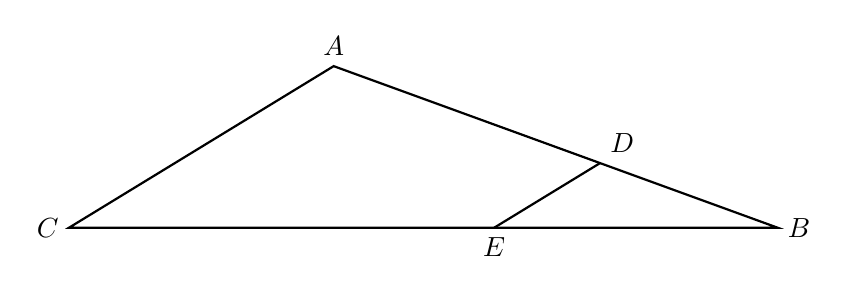
\begin{tikzpicture}[scale=0.6]
  \draw [thick]
  (0,0) node[right] {$B$}--
  (160:10) node[above] {$A$}--
  (-15,0) node[left] {$C$}--cycle;
  \draw [thick]
  (160:4) node[above right] {$D$}--
  (-6,0) node[below] {$E$};
\end{tikzpicture}
\end{center}
IF $EB$ is 3 more than $DB$, $AB=14$, and $CB=21$, what is the length of $\overline{AD}$?

\newpage
\item In the diagram below of $\triangle RST$, $L$ is a point on $\overline{RS}$, and $M$ is a point on $\overline{RT}$, such that $\overline{LM} \parallel \overline{ST}$.
\begin{center}
\begin{tikzpicture}[scale=0.7]
  \draw [thick]
  (0,0) node[below] {$R$}--
  (45:10) node[above right] {$T$}--
  (4,0) node[below] {$S$}--cycle;
  \draw [thick]
  (45:2.5) node[above] {$M$}--
  (1,0) node[below] {$L$};
\end{tikzpicture}
\end{center}
If $RL=2$, $LS=6$, $LM=4$, and $ST=x+2$, what is the length of $\overline{ST}$?

\newpage
\[ f(n) =
  \begin{cases}
    n/2       & \quad \text{if } n \text{ is even}\\
    -(n+1)/2  & \quad \text{if } n \text{ is odd}
  \end{cases}
\]

\end{enumerate}
\end{document}
  